
%(BEGIN_QUESTION)
% Copyright 2014, Tony R. Kuphaldt, released under the Creative Commons Attribution License (v 1.0)
% This means you may do almost anything with this work of mine, so long as you give me proper credit

Apply the concepts of {\it dependability}, {\it security}, {\it PFD}, and {\it RSA} to the context of a firearm.  Label each quadrant of the following chart with these terms (note: some of them may be synonymous, and not all quadrants may have an appropriate term in this list!):

$$\includegraphics[width=15.5cm]{i03021x01.eps}$$

Which of these quadrants represents desirable conditions, and which represent undesirable conditions?  Are there any laws of probability applicable to the quadrants, assuming we had probability values associated with each?

\underbar{file i03021}
%(END_QUESTION)





%(BEGIN_ANSWER)

$$\includegraphics[width=15.5cm]{i03021x02.eps}$$

Probability values in the same column but in different rows (e.g. RSA versus PFD) are {\it mathematical complements} of each other, because their sum must be equal to 100\% (1).  For example, an RSA of 99.98\% is equivalent to a PFD of 0.02\% because there are only two (exclusive) possibilities of what will happen when the trigger is pulled and the safety is off: either the gun will fire or it will not fire.
 
%(END_ANSWER)





%(BEGIN_NOTES)


%INDEX% Safety, system reliability: dependability
%INDEX% Safety, system reliability: probability of failure on demand (PFD)
%INDEX% Safety, system reliability: required safety availability (RSA)
%INDEX% Safety, system reliability: security

%(END_NOTES)


